\documentclass[letterpaper,11pt]{article}
\usepackage[textheight=8in]{geometry}  %excellent for formatting 
\usepackage{graphicx}
\usepackage{natbib}
\usepackage{hyperref}
\hypersetup{citecolor=blue,colorlinks=true,linkcolor=blue,urlcolor=blue}

\begin{document}

\title{\vspace{-0.5in} Simple Stata Exercise}
\author{Tomas Dvorak\thanks{Union College, dvorakt@union.edu}}

\maketitle

\section{Introduction}
The purpose of this exercise is to illustrate the use programming code to perform empirical analysis from beginning to end: from database retrieval, through cleaning and manipulating data, to analysis and display of empirical results. It is inspired by the need to promote reproducible research as outlined in \cite{ball2012teaching}, \cite{gentzkow2014code} and \cite{hoffler2017replication}. 

\section{Data}

The data comes from \href{http://databank.worldbank.org/data/reports.aspx?source=world-development-indicators&preview=on}{World Development Indicators} (WDI) which contains country level annual data on a large number of macroeconomic indicators. The advantage of using WDI is that the data is collected using consistent methodologies. The drawback is that WDI public debt data begins only in 1990 for most countries. 

The descriptive statistics are here:

\input{tables_figures/tab_descriptive_stats}


\section{Is Debt Related to Growth?}
\subsection{Contemporaneous relationship}

\begin{figure}[h!]
\centering
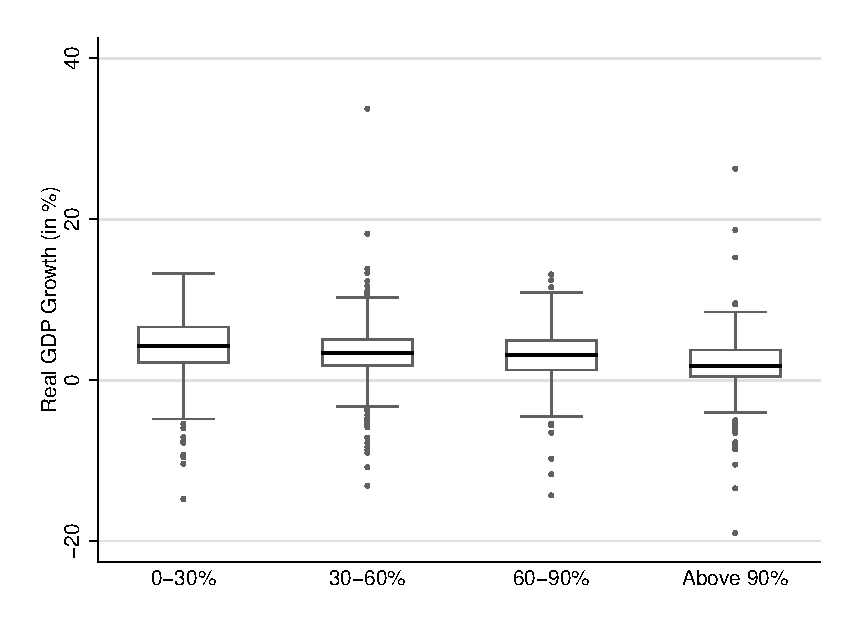
\includegraphics[height=3.5in,]{tables_figures/fig_box_annual.eps}
\caption{Contemporaneous relationship between debt and growth}
\end{figure}

\subsection{Does debt \emph{predict} low growth?}

DONE in more advanced example \href{https://github.com/dvorakt/TIER_debt_growth}{here}.

\section{Conclusion}

You can write it. 

\bibliographystyle{aea}
\bibliography{debtandgrowth}

\end{document}

